\documentclass{BHCexam}
\biaoti{~$2013 - 2014$~学年度第一学期期中考试}
\fubiaoti{高一数学试卷}

\begin{document}
\maketitle
%\mininotice
\notice
\begin{questions}

%选择题
\xuanze
\question 已知函数~$f(x)=\dfrac{1}{\sqrt{1-x}}$~的定义域为~$M$~,~$g(x)=\ln(x+1)$~的定义域为~$N$~,则~$M\cap N$~等于\xx.\\
\onech{$\{x | -1<x<1 \}$}{$\{x|x<1 \}$}{$\{x|x>1 \}$}{$\varnothing$}
\question 已知函数~$ \Bigg\{\begin{aligned}
&\log_2 x,x>0 \\
&3^x,x\leqslant 0
\end{aligned} $~,则~$f[f(\dfrac{1}{4})]$~的值是\xx.\\
\onech{$9$}{$-9$}{$\dfrac{1}{9}$}{$-\dfrac{1}{9}$}
\question 已知~$f(\sqrt{2x-1}+1)=x$~,则\xx.\\
\twoch{$f(x)=x$}{$f(x)=\dfrac{1}{2} x^2-x+1$}{$f(x)=x(x\geq 1)$}{$f(x)=\dfrac{1}{2} x^2-x+1(x\geq 1)$}
\question 下列各不等式中正确的是\xx.\\
\twoch{$\left(\dfrac{1}{2} \right)^{\dfrac{2}{3}}<\left(\dfrac{1}{5} \right)^{\dfrac{2}{3}}<\left(\dfrac{1}{2} \right)^{\dfrac{1}{3}}$}
{$\left(\dfrac{1}{5} \right)^{\dfrac{2}{3}}<\left(\dfrac{1}{2} \right)^{\dfrac{2}{3}}<\left(\dfrac{1}{2} \right)^{\dfrac{1}{3}}$}
{$\left(\dfrac{1}{5} \right)^{\dfrac{2}{3}}<\left(\dfrac{1}{2} \right)^{\dfrac{1}{3}}<\left(\dfrac{1}{2} \right)^{\dfrac{2}{3}}$}
{$\left(\dfrac{1}{2} \right)^{\dfrac{1}{3}}<\left(\dfrac{1}{2} \right)^{\dfrac{2}{3}}<\left(\dfrac{1}{5} \right)^{\dfrac{2}{3}}$}
\question  已知~$ \Bigg\{\begin{aligned}
&1(x\geq 0) \\
&0(x<0)
\end{aligned} $~,则不等式~$xf(x)+x\leq 2$~的解集为\xx.\\
\onech{$(-\infty,1]$}{$[0,2]$}{$(-\infty,2]$}{$[0,1]$}
\question 函数~$f(x)=\ln x-\dfrac{2}{x}$~的零点所在的大致区间是\xx.\\
\onech{$(1,2)$}{$(2,3)$}{$(\dfrac{1}{e},1)$和$(3,4)$}{$(e,+\infty)$}
\question 已知集合~$A=\{x|x<a \},B=\{x|1<x<2 \},A\cup (\complement_R B)=R$~,则实数~$a$~的取值范围是\xx.\\
\onech{$a\geq 2$}{$a>2$}{$a\leq 1$}{$a<1$}
\question 函数~$y=a^{\abs{x}}(a>1)$~的图象是\xx.\\
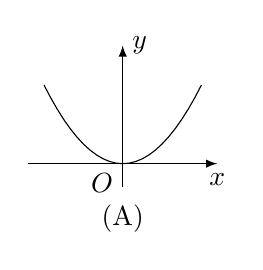
\begin{tikzpicture}
\coordinate[label=below left:$O$] (O) at(0,0);
\draw[->,>=latex](-1.2,0)--(1.2,0)node[below](x){$x$};
\draw[->,>=latex](0,-0.3)--(0,1.5)node[right](y){$y$};
\draw[domain=-1:1]plot(\x,{2 (\x)^2});
\coordinate[label=below:$(\mathrm{A})$] (A) at(0,-0.4);
\end{tikzpicture}
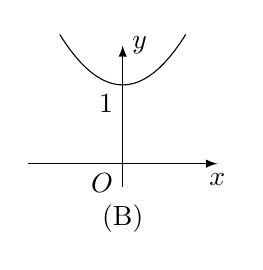
\begin{tikzpicture}
\coordinate[label=below left:$O$] (O) at(3,0);
\draw[->,>=latex](1.8,0)--(4.2,0)node[below](x){$x$};
\draw[->,>=latex](3,-0.3)--(3,1.5)node[right](y){$y$};
\draw[domain=2.2:3.8]plot(\x,{(\x-3)^2+1});
\node[below left](a) at (3,1) {$1$};
\coordinate[label=below:$(\mathrm{B})$] (B) at(3,-0.4);
\end{tikzpicture}
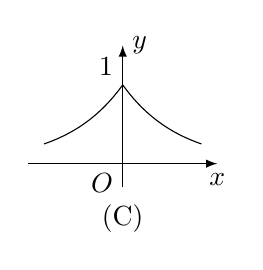
\begin{tikzpicture}
\coordinate[label=below left:$O$] (O) at(6,0);
\draw[->,>=latex](4.8,0)--(7.2,0)node[below](x){$x$};
\draw[->,>=latex](6,-0.3)--(6,1.5)node[right](y){$y$};
\draw[domain=6:7]plot(\x,{(1/4)^(\x-6)});
\draw[domain=5:6]plot(\x,{(1/4)^(6-\x)});
\node[above left](a) at (6,1) {$1$};
\coordinate[label=below:$(\mathrm{C})$] (C) at(6,-0.4);
\end{tikzpicture}
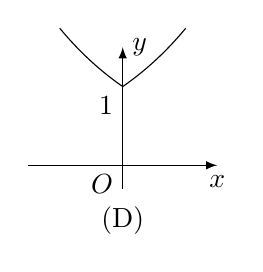
\begin{tikzpicture}
\coordinate[label=below left:$O$] (O) at(9,0);
\draw[->,>=latex](7.8,0)--(10.2,0)node[below](x){$x$};
\draw[->,>=latex](9,-0.3)--(9,1.5)node[right](y){$y$};
\draw[domain=9:9.8]plot(\x,{2^(\x-9)});
\draw[domain=8.2:9]plot(\x,{2^(9-\x)});
\node[below left](a) at (9,1) {$1$};
\coordinate[label=below:$(\mathrm{D})$] (D) at(9,-0.4);
\end{tikzpicture}	
\question 已知函数~$f(x)$~定义域为~$R$~,在~$\big(2010,+\infty \big)$~上是减函数,且函数~$f(x+2010)$~为偶函数,则下列式子正确的是\xx.\\
\twoch{$f(2008)>f(2009)$}{$f(2008)>f(2011)$}{$f(2009)>f(2012)$}{$f(2009)>f(2011)$}
\question 非空集合~$G$~关于运算~$\odot$~满足:\ding{192}对任意~$a,b\in G$~,都有~$a\odot b\in G$~;\ding{194}存在~$e\in G$~,使得对一切~$a\in G$~,都有~$a\odot e=e\odot a=a$~,则称集合~$G$~关于运算~$\odot$~为“和谐集”.现给出下列的集合和运算:\\
\ding{192}~$G=\{$非负整数 $\}$~,~$\odot$~为整数的加法;\quad \ding{193}~$G=\{$偶数 $\}$~,~$\odot$~为整数的乘法;\\
\ding{194}~$G=\{$二次三项式 ~$\}$~,~$\odot$~为多项式的加法.\\
其中~$G$~关于运算~$\odot$~为“和谐集”的是\xx.\\
\onech{\ding{192}}{\ding{192} \ding{193}}{\ding{194}}{\ding{192} \ding{193} \ding{194}}
%填空题
\tiankong
\question 若函数~$f(x)=a^x(a>0$且$a\neq 1)$~的反函数的图象过点~$(3,-1)$~,则~$a=$~\mtk{}.
\question 已知~$f(x)=ax^{2013}+bx^{2011}+cx^{2009}+5(a,b,c\in R)$~.若~$f(\lg2)=10$~,则~$f(\lg \dfrac{1}{2})=$~\mtk{}.
\question 已知函数~$f(x)$~的定义域为~$[0,2]$~,则函数~$g(x)=\dfrac{f(2x)}{x-1}$~的定义域为\mtk{}.
\question 已知函数~$f(x)=\dfrac{\sqrt[3]{8x-1}}{ax^2+x-3}$~的定义域为~$R$~,则实数~$a$~的取值范围是\mtk{}.
\question 某企业年初有资金~$100$~万元,若该企业经过有效经营,能使每年资金平均增长~$50 \%$~,但每年年底要扣除消费基金~$x$~万元,余下的投入再生产,为实现~$3$~年后资金达~$290$~万元(扣除消费基金后),则~$x=$~\mtk{}.

%解答题
\jianda
\question[12] 已知~$x\in R$~,集合~$A=\{ x|x^2-3x+2=0 \},B=\{ x|x^2-3x-2m=0 \}$~,若~$A\cap B=B$~,求实数~$a$~的取值范围.
\vspace{3cm}
\question[12]已知函数~$f(x)=2x-\dfrac{a}{x}(a>0)$~.
\begin{parts}
\part 判断函数~$f(x)$~的奇偶性,并证明你的结论;
\part 求证:函数~$f(x)$~在~$(0,+\infty)$~上是增函数.
\end{parts}
\vspace{6cm}
\question[12] 化简下列各式.
\begin{parts}
\part $4^{\frac{1}{2}}+2\log_4 9-\log_2 \frac{9}{8}$;
\part $(2a^{\frac{2}{3}}b^{\frac{1}{2}})(-6a^{\frac{1}{2}}b^{\frac{1}{3}})\div (-3a^{\frac{1}{6}}b^{\frac{5}{6}})(a>0,b>0)$.
\end{parts}
\vspace{5cm}
\question[13] 已知~$f(x)= \Bigg\{\begin{aligned}
& f_1(x),x\in \left[0,\dfrac{1}{2} \right]\\
&f_2(x),x\in \left(\dfrac{1}{2},1 \right]
\end{aligned} $~,其中~$f_1(x)=-2x^2+2x+\dfrac{1}{2},f_2(x)=-2x+2$~.
\begin{parts}
\part 画出函数~$f(x)$~的图象.
\part 若~$x_0\in \left[0,\dfrac{1}{2} \right],x_1=f(x_0),x_0=f(x_1)$~,求~$x_0$~的值.
\end{parts}
\begin{flushright}
\begin{tikzpicture}
\draw[->] (-1,0) -- (4,0) node[below](x) {$x$};
\draw[->] (0,-1) -- (0,4.5) node[right](y) {$y$};
\draw (0,2) -- (0.1,2);
\draw (0,4) -- (0.1,4);
\draw (1.5,0) -- (1.5,0.1);
\draw (3,0) -- (3,0.1);
\node [below](a) at(1.5,0) {$0.5$};
\node [below](b) at(3,0) {$1$};
\node [left](c) at(0,2) {$0.5$};
\node [left](d) at(0,4) {$1$};
\node [below left] at(0,0) {$O$};
\end{tikzpicture}
\end{flushright}

%\vspace{5cm}
\question[13] 设函数~$f(x)= \begin{cases}
2^{-x+3}~,~x<-1 \\
2^{3x+1}~,~-1\leq x\leq 1 \\
2^{x+3}~,~x>1
\end{cases}$
\begin{parts}
\part 求函数~$f(x)$~的单调区间;
\part 若对任意~$x\in R$~不等式~$f(x)\geq 2^{2a}-2^a-\dfrac{7}{4}$~恒成立,求实数~$a$~的取值范围.
\end{parts}
\vspace{6cm}
\question[13] 已知函数:$f(x)=\log_4 (x+1)+\log_4 (3-x),g(x)=\log_4 (ax^2+2x+3)$.
\begin{parts}
\part 求~$f(x)$~的单调区间;
\part 是否存在非零实数~$a$~,使~$g(x)$~的最小值为~$0$~?若存在。求出~$a$~的值;若不存在,说明理由.
\end{parts}

\end{questions}
\end{document}
